\subsection{Star}%
\label{sub:star}
Ziel von Star ist die Berechnung von gereinigten Kamerabildern und die Berechnung
der Image Parameter auf den Daten.

\paragraph{Theorie}
Sobald das Teleskop ein Event triggert,
speichert es Daten von jedem PMT.\@
Diese Daten enthalten neben dem eigentlichen Tscherenkowlicht auch
Rauschen von elektronischen Bauteilen,
Nachthimmelhintergrund (NSB:\ Night Sky Background) z.B.\ des Mondes,
und andere Störungen.

\subparagraph{Image Cleaning}
Um sinnvoll die Image Parameter bestimmen zu können,
müssen die Daten bereinigt werden.
Dazu werden alle Pixel verworfen, die wahrscheinlich nicht zu den
vom Tscherenkowschauer ausgelösten Pixeln gehören.
Des Weiteren ist gutes Image Cleaning in der Lage,
% um einen konstanten Photostream zu bereinigen,
niederenergetische Ereignisse vom Untergrund zu trennen und damit
für einen geringen Energie-Schwellwert zu sorgen.

Zu jeder anvisierten Quellposition (\textit{On}) werden
genau so lang Daten aufgenommen,
wo kein Gammafluss (\textit{Off}) erwartet wird.
Da insbesondere der NSB abhängig von der Zeit und Quellposition ist,
müssen bei jeder Observation zusätzliche Off-Daten aufgenommen werden.

Das aktuell angewandte Image Cleaning heißt \textit{Sum Image Cleaning}.
Es besteht aus drei Schritten.
Zuerst werde die Pixel zu Clustern aus 2--4 nächsten Nachbarn zusammengefasst.
Es wird überprüft, ob die Summe an Photonen in einem Cluster
einen gewissen clustergrößenabhängigen Grenzwert übersteigt.
Ist dies der Fall, überstehen die Pixel das Cleaning.
Als zweites werden Schnitte auf der Ankunftszeit der so entstandenen
Pixel-Inseln gemacht.
Es werden die mittleren Ankunftszeiten jeder Insel bestimmt.
Weichen die Ankunftszeiten der Inseln zu stark von der Ankunftszeit der größten Insel ab,
werden die Pixel der Insel verworfen.
Pixel der übrigbleibenden Inseln werden im dritten Schritt gereinigt,
wobei zwei Grenzwerte $Q_{1} > Q_{2}$ existieren.
Im ersten Schritt wird geprüft,
ob die Pixel über dem
Grenzwert $Q_{1}$ liegen,
und ob sie einen Cluster mit mindestens zwei Pixeln bilden.
Ist dies der Fall,
werden zusätzlich angrenzende Pixel,
die über dem Grenzwert $Q_{2}$ liegen,
hinzugefügt.

Jeweils ein Beispiel für ein Kamerabild vor und nach dem Image Cleaning ist in
Abbildung~\ref{fig:cleaning} dargestellt.

\begin{figure}[htpb]
  \centering
  \begin{subfigure}[c]{0.35\linewidth}
    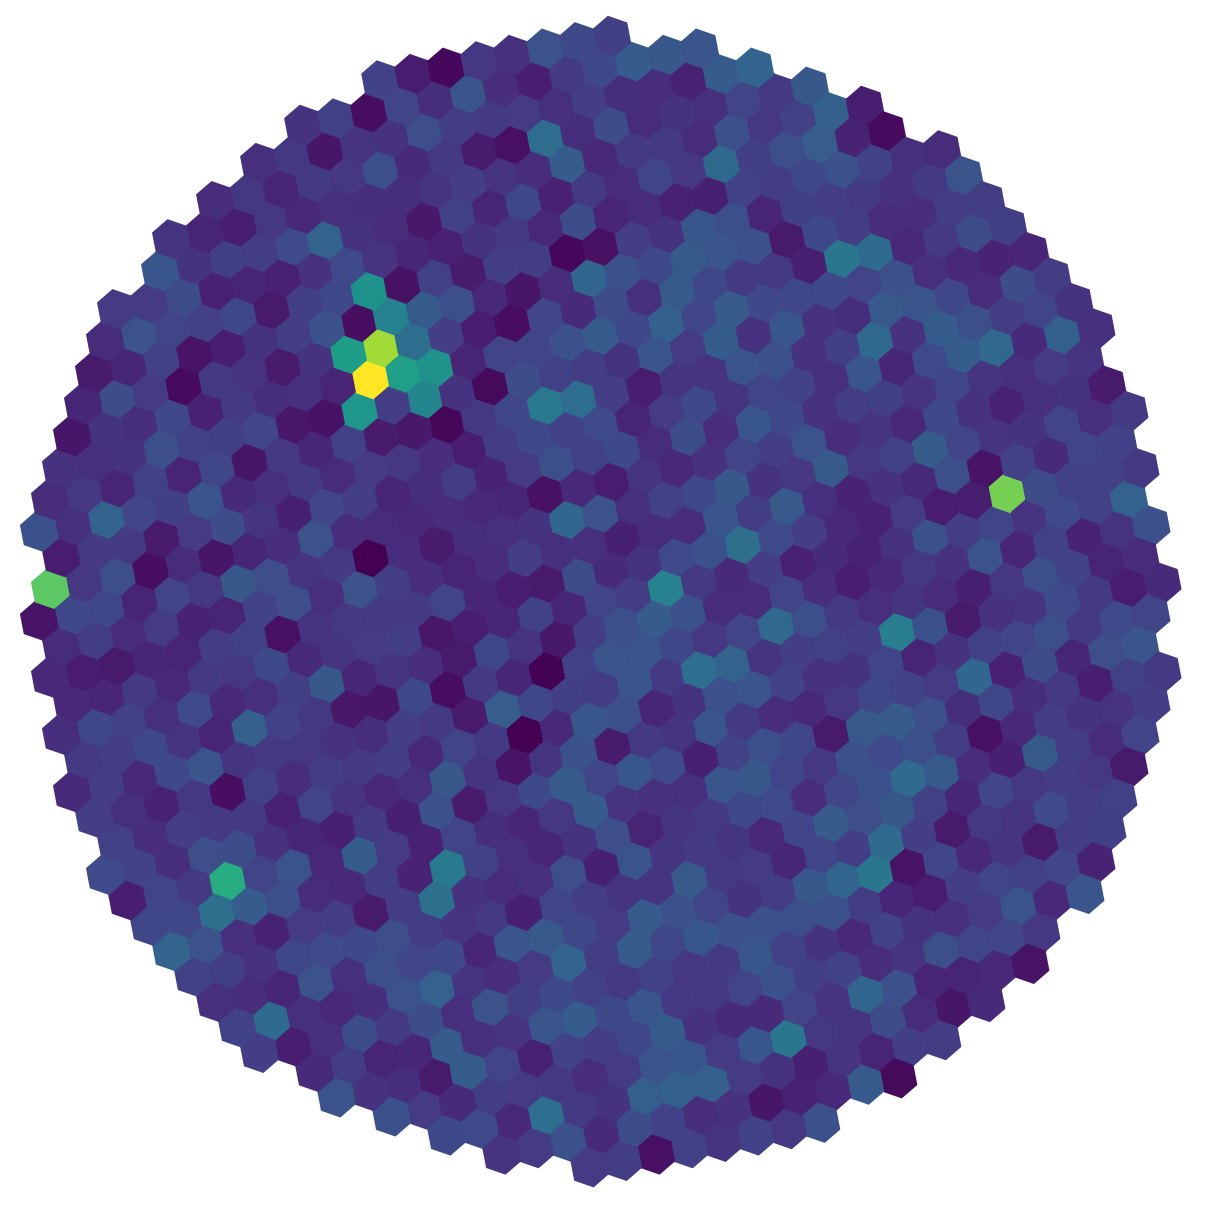
\includegraphics[width=\linewidth]{pictures/uncleaned.png}
    \caption{Kamerabild.}%
    \label{fig:uncleaned}
  \end{subfigure}
	\hspace{1cm}
  \begin{subfigure}[c]{0.35\linewidth}
    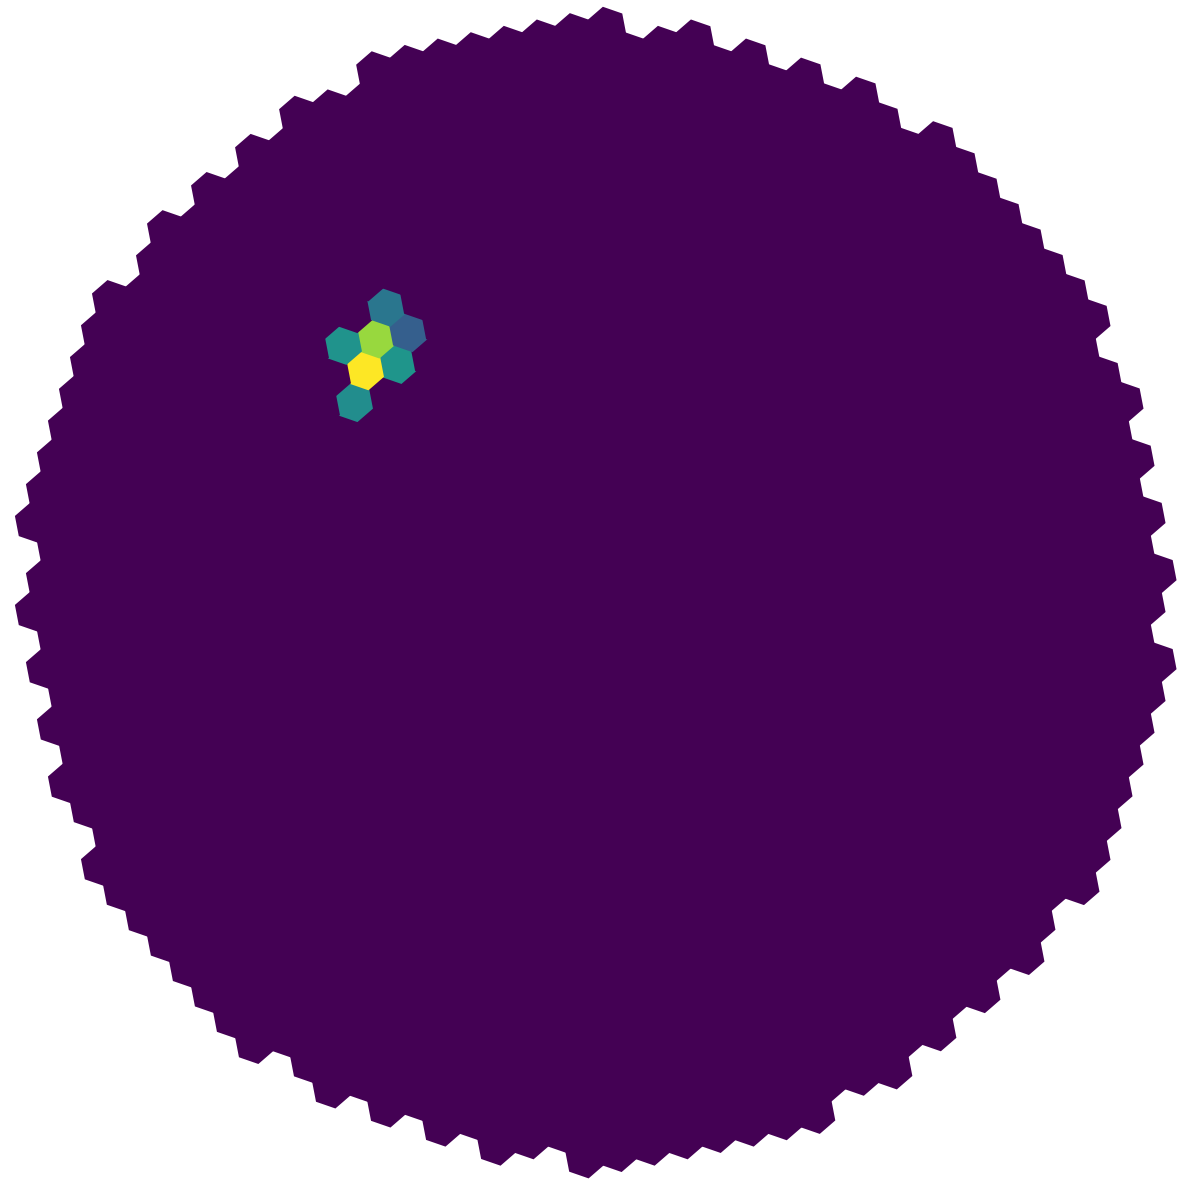
\includegraphics[width=\linewidth]{pictures/cleaned.png}
    \caption{Bereinigtes Kamerabild.}%
    \label{fig:cleaned}
  \end{subfigure}
  \caption{Bereinigung der Kamerabilder zur Berechnung der Image Parameter.}%
  \label{fig:cleaning}
\end{figure}

\subparagraph{Image Parameter}%
\label{spar:image_parameter}

Tscherenkowschauer erzeugen in der Kamera ellipsenförmige Events.
Unter anderem anhand der Größe der Ellipse und deren Ausrichtung
lässt sich die Energie des
Primärteilchens bestimmen und die Richtung rekonstruieren.
Dazu werden auf den gereinigten Kamerabildern die Image Parameter bestimmt.
Die Image Parameter entsprechen teilweise den Hillas Parametern,
und sind zweckmäßig erweitert.


\begin{wrapfigure}[19]{O}{0.6\textwidth}
  \centering
  \includegraphics[width=\linewidth]{tikz/build/imgParam.pdf}
  \caption{Image Parameter eines Schauers.}%
  \label{fig:hillas}
\end{wrapfigure}

Die Image Parameter \textit{length} und \textit{width} geben die Hauptachsen
der Ellipse an.
Da hadronische Schauer höhere transversale Entwicklung zeigen, ist
\textit{width} dazu geeignet, sie von Gammaschauern zu trennen.
\textit{Size} beschreibt die gesamte Anzahl an Photoelektronen im Schauerbild.
Die Anzahl an Photoelektronen verhält sich proportional zur Energie des
Primärteilchens.
\textit{CoG} (Center of Gravity) beschreibt den Schauerschwerpunkt im Kamerabild.
\textit{Conc-n} ist der Anteil der Photoelektronen in den $n$ hellsten Pixeln,
und beschreibt somit die Kompaktheit des Schauers.
Da gammainduzierte Schauer sehr kompakt sind, ist dies auch eine gute
Trennvariable für Gamma/Hadron-Separation.
\textit{Leakage1/2} beschreibt den Anteil des Signals in den \textit{1/2} äußeren
Pixelringen.
Dieser Parameter gibt eine Abschätzung,
ob Teile des Schauers außerhalb des Kamerabildes liegen.
\textit{Alpha} beschreibt den Winkel zwischen Hauptachse der Ellipse und
der Linie vom CoG zum Referenzpunkt (z.B.\ erwartete Quellposition).
Da gammainduzierte Schauer Richtung Quelle zeigen,
ist es ebenfalls ein trennstarker Parameter.
\textit{Dist} ist die Entfernung vom CoG zum Referenzpunkt.
